\section{Figures}
\begin{figure}[htbp]
\centering
\begin{subfigure}[b]{.4\textwidth}
	\centering
	\caption{}
	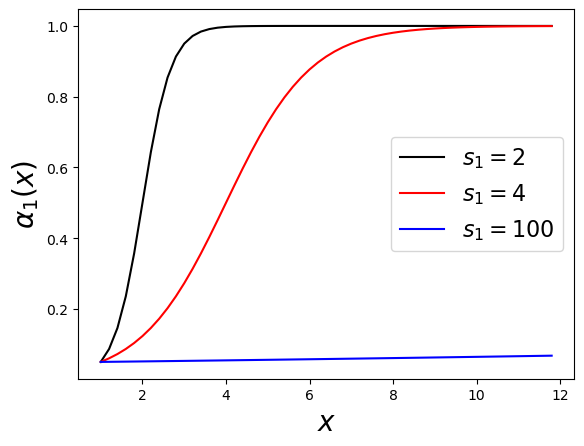
\includegraphics[width=\textwidth]{Figures/capturerate_bigprey.png}
	\label{capture_rates_big}
\end{subfigure}
\begin{subfigure}[b]{.4\textwidth}
	\centering{}
	\caption{}
	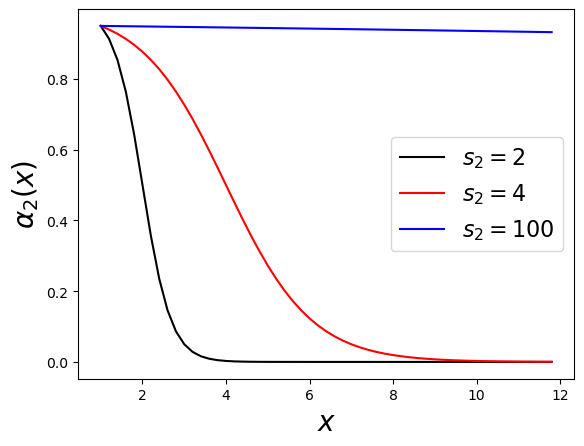
\includegraphics[width=\textwidth]{Figures/capturerate_smallprey.png}
	\label{capture_rates_small}
\end{subfigure}
\caption{Capture probabilities of \textbf{(A)} big prey and \textbf{(B)} small prey where the capture probability for solitary predators if $\alpha_1(1)= 0.05$ for big prey and $\alpha_2(1) = 0.95$ for small prey. In panel \textbf{(A)}, the capture probability is shown for critical group sizes $s_1 = 2$ (black line), $s_1 = 4$ (red line), and $s_1 = 100$ (blue line). Similarly in panel \textbf{(B)}, the capture probability is shown for critical group sizes $s_2 = 2$ (black line), $s_2 = 4$ (red line), and $s_2 = 100$ (blue line)}
\label{default}
\end{figure}